\title{A Pipelined SIMD Vector Processing Unit with\\Masked Execution on FPGA}

\author{Mahir Abdullah, Krishiv Gupta, Abhiman Singh, Gogulamudi Jayadeep, and Ashish Kushwaha%
\thanks{This work forms Phase~II of Project 11, SIMD Vector Processing Unit, November 2026.
The authors are with Newton School of Technology, Rishihood University.}%
\thanks{Code, data and all reported results are available at
\url{https://github.com/mahir-m01/SIMD-Vector-Processing-Unit}.}}

\markboth{A Pipelined SIMD Vector Processing Unit with Masked Execution on FPGA}%
{A Pipelined SIMD Vector Processing Unit with Masked Execution on FPGA}

\maketitle

% =============================================================================
\begin{abstract}
Phase~I of this project built a parameterised SIMD vector processing unit whose
eight 16-bit lanes needed $7.9\x$ fewer clock cycles than one lane, but whose
single-cycle design lost a third of its clock speed as lanes were added, so the
real-time speed-up was only $5.3\x$. Phase~II removes that limit and widens the
instruction set. Timing analysis of the single-cycle core showed its critical
path in three nearly equal parts: instruction fetch and register read, the lane
multiplier, and the adder tree with write-back. We therefore add a four-stage
pipeline (fetch, decode, execute, write) with forwarding, write-through register
files, one-cycle stalls for the three results that cannot be forwarded in time,
and static backward-taken branch prediction. We also add merge-masked execution
for every vector and reduce instruction, a mask-setting instruction, and
saturating addition and subtraction, for 55 instructions. The single-cycle core
is kept with the same instruction set as a like-for-like baseline. An extended
golden model predicts the exact cycle count of both cores, and every workload,
directed test, mid-run reset and random program matches it at 1, 2, 4 and 8
lanes; all 23 deliberately planted pipeline bugs are caught. On a Lattice
ECP5-25F the pipelined core reaches 50.6~MHz at eight lanes against 27.1~MHz for
the single-cycle core, for 39\% more logic. Across eight workloads it is
$1.90\x$ faster in real time at eight lanes and $10.9\x$ faster than the scalar
single-cycle design; with loops unrolled to avoid stalls, $18.6\x$ faster than
the original programs on that design. A size sweep reproduces Amdahl's law: the eight-lane cycle speed-up
falls from $7.9\x$ at 256 elements to $5.0$--$6.1\x$ at eight.
\end{abstract}

\begin{IEEEkeywords}
Data hazards, FPGA, forwarding, masked execution, pipelining, predication,
saturating arithmetic, SIMD, static branch prediction, Verilog.
\end{IEEEkeywords}

% =============================================================================
\section{Introduction}
\IEEEPARstart{D}{ata-level} parallelism is cheap to exploit in hardware: one
instruction, one decoder and one control decision can drive several identical
arithmetic lanes \cite{flynn72, hp6}. Phase~I of this project built such a unit in
Verilog, with the lane count $L$ as a parameter, so that $L = 1$ gives a scalar
processor that runs the same programs as the SIMD versions. Its results framed the
questions for Phase~II. Counted in clock cycles, eight lanes did almost eight times
the work per instruction ($7.87$--$7.92\x$ fewer cycles). Counted in time, they did
not: every instruction finished in one clock, the critical path ran from the
instruction memory through the register file, a lane multiplier and the adder tree
into the scalar register file, and that path lengthened with $L$. The clock fell from
43.3~MHz at one lane to 29.1~MHz at eight, and the wall-clock speed-up was only
$5.3\x$. The unit also lacked two features that real SIMD instruction sets rely on:
a way to act on only some lanes, and arithmetic that saturates instead of wrapping.

Phase~II therefore asks four questions.
\begin{enumerate}
\item Where exactly does the single-cycle core spend its clock period, and what
      pipeline does that suggest?
\item Can the pipeline keep the cycle-exact correctness of Phase~I, including the
      golden-model cycle count, at every lane count?
\item How much of the clock-speed gain survives as real speed-up once the cycles
      the pipeline loses to hazards are counted?
\item How do problem size and the order of the instructions change the answer?
\end{enumerate}

To answer the third question fairly, both cores implement the same extended
instruction set and are built, verified and measured with the same flow; the only
difference between them is the pipeline.

The contributions are: a measured critical-path decomposition of the Phase~I core
(Section~\ref{sec:why}); a four-stage pipelined core with forwarding, write-through
register files, three stall rules and static branch prediction, in which one
forwarding path was removed because the timing report showed it cost more than it
saved (Section~\ref{sec:pipe}); merge-masked execution and saturating arithmetic
across both cores (Section~\ref{sec:isa}); a golden model that predicts the cycle count
of both cores, with a verification campaign that includes planted-bug and mid-run
reset tests (Section~\ref{sec:verif}); and a measured comparison of the two cores in
logic, clock speed, cycles and real time, including problem-size and unrolling studies
(Section~\ref{sec:results}).

% =============================================================================
\section{Literature Review}\label{sec:lit}

\subsection{Pipelining and Hazards}
Pipelining overlaps the execution of successive instructions in stages separated by
registers, so that the clock period covers one stage instead of the whole
instruction \cite{hp6, pattersonrv}. The cost is hazards. A data hazard arises when an
instruction needs a result that an older instruction has not yet written; the classic
five-stage RISC pipeline resolves most of them by forwarding results from later stages
to the inputs of the execute stage, and stalls for one cycle when a load's data is used
by the very next instruction, because that data arrives too late to forward
\cite{pattersonrv}. Writing the register file in the first half of the cycle and
reading it in the second half removes the hazard between instructions two apart; a
write-through (bypassing) register file achieves the same with a multiplexer per read
port. A control hazard arises because the next instruction must be fetched before a
branch is resolved. Static prediction guesses without history; among the strategies Smith
compared is to predict backward branches taken and forward branches not taken (BTFN)
\cite{smith81}, which suits loops, whose closing branch is backward and almost always
taken, and needs only the sign of the offset. Dynamic
predictors do better on irregular code but need tables, which a small loop-dominated
accelerator does not justify.

\subsection{Predication and Masked Execution}
Conditional code in data-parallel loops cannot branch per lane. If-conversion turns
control dependence into data dependence: both outcomes are computed and a predicate
selects between them \cite{allen83}. Packed SIMD extensions such as SSE and NEON do
this with compare results used as bit masks and explicit blend or select instructions
\cite{sse, armarm}; Phase~I followed that convention. Vector architectures instead
predicate the instruction itself: the Cray-1 had a vector mask register \cite{cray1},
RISC-V V masks any instruction with register \texttt{v0} \cite{rvv}, ARM SVE has
sixteen predicate registers \cite{sve} and AVX-512 eight opmask registers \cite{intelsdm}.
Two policies exist for the inactive lanes: merging keeps their old destination value,
zeroing clears them. Merging needs the old value, which in hardware means either an
extra register-file read port or per-lane write enables.

\subsection{Saturating Arithmetic}
Media instruction sets added saturating addition because wrap-around is the worst
possible answer for pixels and audio samples: a bright pixel that overflows becomes
black \cite{mmx}. Signed saturating addition is now standard in SSE2, NEON, MSA and
RISC-V V \cite{intelsdm, armarm, msa, rvv}.

\subsection{Soft Vector Processors on FPGAs}
FPGA soft vector processors such as VESPA \cite{vespa}, VIPERS \cite{vipers}, VEGAS
\cite{vegas} and MXP \cite{mxp} map lane-replicated, pipelined datapaths onto FPGA DSP
blocks and block RAM. Our unit is far smaller, but it meets the same structures in its
timing: the block-RAM access time and the cross-lane adder tree dominate its
single-cycle path (Section~\ref{sec:why}).

\subsection{Instruction Scheduling and Problem Size}
Stalls in an in-order pipeline can be removed in software by placing independent
instructions between a producer and its consumer; loop unrolling both creates such
independent instructions and amortises the loop overhead \cite{dongarra79, hp6}.
Amdahl's law bounds the speed-up from parallel lanes by the fraction of work that does
not scale with them \cite{amdahl}; with fixed setup code, that fraction depends on the
problem size, which Gustafson pointed out for scaled problems \cite{gustafson}.

% =============================================================================
\section{Proposed Solution}\label{sec:design}

\subsection{Where the Single-Cycle Core Spends Its Clock}\label{sec:why}
We read the critical path of the Phase~I eight-lane build from nextpnr's timing report
(ECP5-25F, speed grade~6, seed~1). It was 34.7~ns long and fell into three nearly equal
parts: instruction fetch, decode and the LUT-RAM register read, about 12.8~ns together
(5.6~ns of it the block RAM's clock-to-output time); the lane multiplier and its result
multiplexer, about 9~ns; and the three-level adder tree of the reduction with the write
into the scalar register file, about 12.7~ns. Three balanced pieces suggest registers
between them, which gives the four-stage pipeline of Fig.~\ref{fig:pipe}.

\subsection{Instruction Set Extensions}\label{sec:isa}
Phase~II keeps the Phase~I encoding (Table~\ref{tab:isa2}) and fills its spare space.
\emph{Saturating jobs.} The last two free ALU job codes become \texttt{ADDS} and
\texttt{SUBS}, available in all three forms (vector--vector, vector--scalar and reduce).
The lane computes the sum with one extra bit, so it can never overflow; when the top two
bits of the 17-bit result differ, the true value lies outside $[-32768, 32767]$ and the
top bit selects the limit.
\emph{Masked execution.} Bit~16, unused in Phase~I, marks a vector or reduce
instruction as masked (\texttt{.M} in the assembler). A masked vector instruction
merges: lanes whose mask bit is 0 keep the old value of $v_d$. A masked reduction adds
only the active lanes. \texttt{VMSK} $v_a$ sets the mask register to one bit per lane,
$m_i = [v_a[i] \neq 0]$, so a compare followed by \texttt{VMSK} activates exactly the
lanes where the compare was true. The mask resets to all ones at power-up.
Merging is implemented with per-lane write enables in the vector register file, so no
third read port is needed; \texttt{VMSK} reuses the lanes (it executes as
$v_a \,|\, s_0$, with $s_0 = 0$) and the result combiner, which flags the non-zero lanes.

\begin{table}[t]
\centering
\caption{Instruction set after Phase~II (55 instructions)}
\label{tab:isa2}
\footnotesize
\begin{tabular}{@{}lll@{}}
\toprule
Opcodes & Instruction & Phase~II change \\
\midrule
\texttt{0x00}--\texttt{0x0F} & $v_d = v_a \circ v_b$ & jobs 14, 15: \texttt{ADDS}, \texttt{SUBS} \\
\texttt{0x10}--\texttt{0x1F} & $v_d = v_a \circ s_b$ (broadcast) & same; all forms maskable \\
\texttt{0x20}--\texttt{0x2F} & $s_d = \sum_i (v_a \circ v_b)_i$ & masked: active lanes only \\
\texttt{0x30}, \texttt{0x31} & \texttt{VLD}, \texttt{VST} & -- \\
\texttt{0x34} & \texttt{VMSK} $v_a$ & new: mask $= [v_a \neq 0]$ \\
\texttt{0x38}, \texttt{0x39} & \texttt{ADDI}, \texttt{ADD} & -- \\
\texttt{0x3C}, \texttt{0x3F} & \texttt{BNE}, \texttt{HALT} & -- \\
\midrule
bit 16 & mask flag (classes \texttt{00}--\texttt{10}) & new; ignored in class \texttt{11} \\
\bottomrule
\end{tabular}
\end{table}

\begin{figure*}[t]
\centering
% Pipelined core: four stages, three pipeline registers, and the paths that
% handle hazards (forwarding, write-through, branch guess and check, stall).
% Blue = vector datapath, orange = scalar side, grey = control and memories.
% Dashed = control.
\begin{tikzpicture}[x=1mm, y=1mm, font=\footnotesize,
    blk/.style={box, minimum height=9mm, inner sep=2pt},
    vblk/.style={blk, fill=simdfill, draw=simd},
    sblk/.style={blk, fill=scalfill, draw=scal},
    gblk/.style={blk, fill=greyfill},
    preg/.style={draw=edge, fill=greyfill, minimum width=2.6mm, minimum height=56mm, inner sep=0pt},
    stage/.style={font=\small\bfseries, text=edge},
    lbl/.style={note}]

% ---- Stage titles and pipeline registers ----------------------------------------
\node[stage] at (9,50)   {F: fetch};
\node[stage] at (50,50)  {D: decode};
\node[stage] at (107,50) {X: execute};
\node[stage] at (157,50) {W: write};

\node[preg] (fd) at (24,4) {};  \node[lbl, above=0.5mm] at (fd.north) {RAM out};
\node[preg] (dx) at (78,4) {};  \node[lbl, above=0.5mm] at (dx.north) {D/X};
\node[preg] (xw) at (136,4) {}; \node[lbl, above=0.5mm] at (xw.north) {X/W};

% ---- F ---------------------------------------------------------------------------
\node[gblk, minimum width=17mm] (imem) at (9,14)  {Instruction\\memory};
\node[gblk, minimum width=17mm] (fsel) at (9,-14) {Next fetch\\address};

% ---- D ---------------------------------------------------------------------------
\node[gblk, minimum width=24mm] (dec)  at (42,24)  {Decoder};
\node[gblk, minimum width=13mm] (guess) at (66,24) {Branch\\guess};
\node[vblk, minimum width=34mm] (vrf)  at (51,9)   {Vector registers + mask\\\scriptsize write-through};
\node[sblk, minimum width=34mm] (srf)  at (51,-4)  {Scalar registers\\\scriptsize write-through};
\node[gblk, minimum width=34mm] (haz)  at (51,-14) {Hazard unit\\\scriptsize stall $\cdot$ forwarding select};

% ---- X ---------------------------------------------------------------------------
\node[vblk, minimum width=7mm, minimum height=26mm, font=\scriptsize] (fwd) at (87,4) {};
\node[font=\scriptsize, rotate=90] at (fwd.center) {forwarding select};
\node[vblk, minimum width=14mm] (mux)  at (102,13) {Lane\\MUX};
\node[vblk, minimum width=16mm] (alus) at (122,13) {8 lane\\ALUs};
\node[sblk, minimum width=14mm] (sadd) at (102,-4) {Scalar\\adder};
\node[gblk, minimum width=16mm] (dmem) at (122,-4) {Data\\memory};
\node[gblk, minimum width=14mm] (bchk) at (102,-17){Branch\\check};

% ---- W ---------------------------------------------------------------------------
\node[vblk, minimum width=26mm] (comb) at (157,13) {Result combiner\\\scriptsize adder tree $\cdot$ lane flags};
\node[gblk, minimum width=26mm] (wsel) at (157,-6) {Result select\\\scriptsize lanes / sum / load};

% ---- Main flow -------------------------------------------------------------------
\draw[arr] (imem.east) -- (fd.west |- imem.east);
\draw[arr] (fd.east |- dec.west) -- (dec.west);
\draw[arr] (dec.south) -- (dec.south |- vrf.north);
\draw[arr] (vrf.east) -- (dx.west |- vrf.east);
\draw[arr] (srf.east) -- (dx.west |- srf.east);
\draw[arr] (dx.east |- 0,13) -- (fwd.west |- 0,13);
\draw[arr] (dx.east |- 0,-4) -- (fwd.west |- 0,-4);
\draw[arr] (fwd.east |- mux.west) -- (mux.west);
\draw[arr] (mux.east) -- (alus.west);
\draw[arr] (fwd.east |- sadd.west) -- (sadd.west);
\draw[arr] (sadd.east) -- node[above, lbl]{addr} (dmem.west);
\draw[arr] (fwd.east |- 0,-7) -- (94,-7) |- (bchk.west);
\draw[arr] (alus.east) -- (xw.west |- alus.east);
\draw[arr] (dmem.east) -- (xw.west |- dmem.east);
\draw[arr] (xw.east |- comb.west) -- (comb.west);
\draw[arr] (xw.east |- wsel.west) -- node[above, lbl, pos=0.45]{load} (wsel.west);
\draw[arr] (comb.south) -- (wsel.north);

% ---- Forwarding: W back to the operands in X ----------------------------------------
\draw[arr, draw=simd, line width=0.8pt] (wsel.east) -- (176,-6) -- (176,38) -- node[above, lbl, pos=0.5]{forwarding: the result in W replaces a stale operand in X} (87,38) -- (fwd.north);

% ---- Write-back into the register files, seen at once in D ----------------------------
\draw[arr, draw=simd, line width=0.8pt] (wsel.south) -- (157,-35) -- node[below, lbl, pos=0.5]{write-back; write-through makes it visible to D in the same cycle} (30,-35) -- (30,9) -- (vrf.west);
\draw[arr, draw=scal, line width=0.8pt] (30,-4) -- (srf.west);

% ---- Branches and stalls --------------------------------------------------------------
\draw[arr, dashed] (dec.east) -- (guess.west);
\draw[arr, dashed] (guess.north) -- (66,41) -- node[above, lbl, pos=0.55]{backward branch: fetch its target next} (2,41) -- (2,-14) -- (fsel.west);
\draw[arr, dashed] (bchk.south) -- (102,-28) -- node[below, lbl, pos=0.45]{wrong guess: drop the instruction in D, fetch the right one} (9,-28) -- (fsel.south);
\draw[arr, dashed] (haz.west) -- node[below, lbl, pos=0.15]{stall} (fsel.east |- haz.west);
\draw[arr] (fsel.north) -- node[right, lbl]{address} (imem.south);
\end{tikzpicture}

\caption{The pipelined core. Fetch (F) is the instruction block RAM; decode (D) reads
the write-through register files, guesses backward branches taken and runs the hazard
unit; execute (X) holds the forwarding select, the lane multiplexers and ALUs, the
scalar adder, the data-memory access and the branch check; write (W) adds the lanes for
reductions, flags non-zero lanes for \texttt{VMSK} and selects the value to write. Blue
lines carry the result back: forwarded from W to X, and written through to D.}
\label{fig:pipe}
\end{figure*}

\subsection{Pipeline Organisation}\label{sec:pipe}
The four stages and their registers are shown in Fig.~\ref{fig:pipe}. The instruction
memory's own output register is the boundary between fetch and decode, as in Phase~I,
so the pipeline adds two registers: D/X, which holds the decoded control signals and the
operands read in D, and X/W, which holds the lane results, the scalar adder's result and
the lane enables. One decoder module is shared by both cores; besides the control
signals it lists which registers an instruction reads and writes, which the hazard unit
needs. Every pipeline-register field carries a valid bit, and nothing that changes
state (a memory write, a register write, a branch correction) acts on an invalid entry.

\emph{Data hazards.} Three mechanisms keep results correct. (i) Forwarding: when the
instruction in X reads a register that the instruction in W is writing, it takes the
value from the X/W register instead of the stale copy read in D. (ii) Write-through
register files: an instruction two places behind a producer reads its registers in D
while the producer writes in W; the register files return the value being written in
the same cycle, lane by lane, so nothing more is needed. (iii) Stalls: three kinds of
result are not available at the start of W and are not forwarded
(Table~\ref{tab:stalls}). When the instruction in D needs one of them from the
instruction in X, D holds for one cycle and a bubble enters X; a cycle later the
producer is in W and the write-through file supplies the value.

\begin{table}[t]
\centering
\caption{Results that make the next instruction wait one cycle}
\label{tab:stalls}
\footnotesize
\begin{tabular}{@{}L{1.7cm}L{3.4cm}L{2.5cm}@{}}
\toprule
Producer & Why it is not forwarded & Example \\
\midrule
reduction & the adder tree sums the lanes during W & \texttt{VDOT s4} then \texttt{ADD s3, s3, s4} \\
masked vector op & inactive lanes must keep the old value, held only by the register file & \texttt{VADD.M v3} then \texttt{VST v3} \\
load & data arrives from block RAM during W; forwarding it into the multiplier slowed the clock (Section~\ref{sec:fwdload}) & \texttt{VLD v2} then \texttt{VADD v3, v1, v2} \\
\bottomrule
\end{tabular}
\end{table}

\emph{Control hazards.} Branches are checked in X, against forwarded operands. In D,
a branch with a negative offset is guessed taken and its target is fetched at once;
a forward branch is guessed not taken. A wrong guess turns the one wrongly fetched
instruction in D into a bubble and fetches the correct address, so it costs one cycle;
a loop's branch is wrong only at its exit. The guess uses the sign bit of the full
16-bit offset.

\emph{Halting and reset.} Once \texttt{HALT} leaves D, D stops passing instructions on;
a \texttt{HALT} fetched on a wrong path never leaves D because the wrong guess removes
it first. \texttt{halted} rises when \texttt{HALT} leaves X, at the same clock edge at
which the last older instruction is written in W. Reset invalidates every stage and
blocks every write while it is held.

\emph{Loads.} \texttt{VLD} sends its address in X and writes its data in W, so a load
occupies one cycle instead of the two of the single-cycle core.

\emph{Cycle count.} With these rules the pipelined core needs
\begin{equation}
C_{\mathrm{pipe}} = I + 1 + S + M,
\end{equation}
cycles, where $I$ is the number of instructions executed, the 1 fills the pipeline, $S$
counts stalls and $M$ wrong branch guesses; the single-cycle core needs
$C_{\mathrm{single}} = I + \Lambda$, where $\Lambda$ is the number of loads.
Fig.~\ref{fig:timing} shows one pass of the \texttt{vadd} loop.

\begin{figure*}[t]
\centering
% Pipeline timing of one vadd loop pass on the pipelined core: the
% load-use stall (VADD waits for v2), forwarding (VST gets v3 from W) and the
% backward branch guessed taken (the next pass starts at once).
\begin{tikzpicture}[x=7.4mm, y=5.2mm, font=\scriptsize]
  \tikzset{st/.style={draw=edge, minimum width=6.6mm, minimum height=4.4mm, inner sep=0pt, font=\scriptsize},
           F/.style={st, fill=greyfill}, D/.style={st, fill=simdfill}, X/.style={st, fill=simdfill, draw=simd},
           W/.style={st, fill=white}, B/.style={st, fill=scalfill, draw=scal}}
  % cycle numbers
  \foreach \c in {1,...,10} \node[text=edge] at (\c+1.6, 0.9) {\c};
  \node[text=edge, anchor=east] at (2.0, 0.9) {cycle};
  % instructions (row, label)
  \foreach \r/\t in {0/{VLD v1, A(s1)}, 1/{VLD v2, B(s1)}, 2/{VADD v3, v1, v2}, 3/{VST v3, C(s1)},
                     4/{ADDI s1, s1, 1}, 5/{BNE s1, s2, loop}, 6/{VLD v1, A(s1)}}
     \node[anchor=east, font=\ttfamily\scriptsize] at (2.0, -\r) {\t};
  % stages: \node[style] at (cycle+1.6, -row)
  \node[F] at (2.6,0) {F}; \node[D] at (3.6,0) {D}; \node[X] at (4.6,0) {X}; \node[W] at (5.6,0) {W};
  \node[F] at (3.6,-1) {F}; \node[D] at (4.6,-1) {D}; \node[X] at (5.6,-1) {X}; \node[W] at (6.6,-1) {W};
  \node[F] at (4.6,-2) {F}; \node[D] at (5.6,-2) {D}; \node[B] at (6.6,-2) {D}; \node[X] at (7.6,-2) {X}; \node[W] at (8.6,-2) {W};
  \node[F] at (5.6,-3) {F}; \node[B] at (6.6,-3) {F}; \node[D] at (7.6,-3) {D}; \node[X] at (8.6,-3) {X}; \node[W] at (9.6,-3) {W};
  \node[F] at (7.6,-4) {F}; \node[D] at (8.6,-4) {D}; \node[X] at (9.6,-4) {X}; \node[W] at (10.6,-4) {W};
  \node[F] at (8.6,-5) {F}; \node[D] at (9.6,-5) {D}; \node[X] at (10.6,-5) {X}; \node[W] at (11.6,-5) {W};
  \node[F] at (9.6,-6) {F}; \node[D] at (10.6,-6) {D}; \node[X] at (11.6,-6) {X};
  % notes
  \node[anchor=west, text=scal] at (12.4,-2) {stall: \texttt{v2} is still on its way from memory};
  \draw[arr, draw=simd] (8.6,-2.4) -- (8.6,-2.6);
  \node[anchor=west, text=simd] at (12.4,-3) {forwarded: \texttt{v3} taken from W};
  \node[anchor=west, text=edge] at (12.4,-5) {guessed taken in D \dots};
  \node[anchor=west, text=edge] at (12.4,-6) {\dots\ so the next pass starts at once};
\end{tikzpicture}

\caption{One pass of the \texttt{vadd} loop on the pipelined core. \texttt{VADD} needs
\texttt{v2} one cycle after its load and waits in D (orange); \texttt{VST} receives
\texttt{v3} by forwarding from W; the backward \texttt{BNE} is guessed taken in D, so the
next pass starts without a bubble. The six instructions of a pass take seven cycles,
against eight on the single-cycle core.}
\label{fig:timing}
\end{figure*}

\subsection{A Forwarding Path Removed by Measurement}\label{sec:fwdload}
The first version of the pipeline also forwarded load data, so a load followed at once
by its consumer cost nothing. Its timing report showed the new critical path: the data
block RAM's 5.6~ns clock-to-output, then the forwarding multiplexer, the lane multiplier
and the ALU result multiplexer, all in one cycle. Removing that one path and stalling
instead, as the classic MIPS pipeline does, trades cycles for clock speed
(Table~\ref{tab:fwd}): $F_{\max}$ rises by 18\%, and over the eight workloads the
stall version is faster on six and 4.5\% faster on average. On \texttt{relu} and
\texttt{brighten}, short loops in which every pass has one load-use pair, forwarding is
about 1\% faster. A load followed by an independent instruction pays nothing, which is
why \texttt{saxpy}, whose loaded registers are used two instructions later, gains the
full 18\% and benefits most from the pipeline.

\begin{table}[t]
\centering
\caption{Forwarding load data or stalling (8 lanes, ECP5, median of 3 seeds)}
\label{tab:fwd}
\footnotesize
\begin{tabular}{@{}lrrr@{}}
\toprule
 & $F_{\max}$ & \multicolumn{2}{c}{\texttt{vadd}} \\
\cmidrule(l){3-4}
Version & (MHz) & cycles & $\mu$s \\
\midrule
single-cycle & 27.1 & 259 & 9.57 \\
pipelined, load data forwarded & 42.8 & 197 & 4.61 \\
pipelined, load-use stall (kept) & 50.6 & 229 & 4.53 \\
\bottomrule
\end{tabular}
\end{table}

\subsection{Verification Methodology}\label{sec:verif}
The Phase~I method carries over: every block has a self-checking testbench, and the
whole core is compared with an instruction-level golden model written in Python. The
RTL is Verilog-2005 \cite{ieee1364}, simulated with Icarus Verilog \cite{icarus} and
linted with Verilator \cite{verilator}; synthesis uses Yosys \cite{yosys} and
nextpnr \cite{nextpnr}. The
model now implements masks, \texttt{VMSK} and saturation, and predicts the cycle count
of either core from the rules above: for the pipelined core it decodes each instruction's
read set, applies the three stall rules to each adjacent pair and the BTFN guess to each
branch. Because the model knows nothing about pipeline registers, agreement on the cycle
count is a strong check of the hazard logic: a missed stall corrupts a result, and a
spurious one changes the count.

The system testbench, now parameterised by core, runs a program to \texttt{HALT}, keeps
the clock running for 50 more cycles and compares every data-memory word, every scalar
and vector register, the lane mask, the instruction count and the cycle count with the
model. Around it run: eleven workloads and six directed programs on both cores at
1, 2, 4 and 8 lanes; the directed programs include \texttt{hazards}, which places every
producer right before every kind of consumer and exercises branch guesses in both
directions, a wrong-path \texttt{HALT} and a wrong-path store, \texttt{masks}, and
\texttt{far\_branch}, with offsets far beyond $\pm127$; a reset pressed in the middle of
three restartable programs at ten consecutive cycles, during which no write of any kind
may happen and after which the restarted program must end exactly as a clean run; random
programs on both cores with random mask bits, \texttt{VMSK}, loads, stores and
branches (25 per configuration in \texttt{make test}, 1,000 in \texttt{make fuzz}); and a
board simulation of each core from power-on (Table~\ref{tab:directed}). Mutation analysis \cite{demillo} checks the
tests: we planted 23 bugs in the pipeline one at a time, from switching off each
forwarding path and each stall rule to letting a store through during reset, and each
had to make a test fail. An independent reviewer, given only the repository, tried to
break the design; three of the 23 planted bugs come from that review, which found no bug
in the RTL.

\begin{table}[t]
\centering
\caption{Directed programs (run on both cores at every lane count)}
\label{tab:directed}
\footnotesize
\begin{tabular}{@{}lL{6.2cm}@{}}
\toprule
Program & What it checks \\
\midrule
\texttt{corners} & writes to \texttt{s0}; address wrap; scalar wider than 16 bits broadcast; saturating jobs in all three forms; unused opcodes \\
\texttt{pc\_wrap} & program counter wrapping from 255 to 0 \\
\texttt{branch\_halt} & \texttt{BNE} on bits 16 and 31; unused fields set; nothing after \texttt{HALT} runs \\
\texttt{hazards} & every producer right before every consumer; stalled backward and forward branches; wrong guesses both ways; wrong-path \texttt{HALT} and store \\
\texttt{masks} & mixed, empty and full masks; merges keep old lanes; masked reduce and broadcast \\
\texttt{far\_branch} & branch offsets beyond $\pm127$, guessed right and wrong \\
\bottomrule
\end{tabular}
\end{table}

\subsection{Workloads and Experimental Setup}\label{sec:setup}
Table~\ref{tab:work2} lists the programs. The five Phase~I kernels are unchanged, so both
phases measure identical code; three new kernels use the Phase~II instructions, and two
unrolled versions isolate the effect of instruction order. Every kernel processes
$N = 256$ random 16-bit elements over the full range (fixed seeds, the same data for every
lane count and core), and every result is checked twice: the golden model against plain
Python arithmetic, and the RTL against the golden model.

FPGA results come from the board version of each core, with 256-word instruction and
1,024-word data block RAMs, loaded with the program that uses every instruction. Yosys
synthesises it for the Lattice ECP5-25F (speed grade~6, CABGA256); nextpnr places and
routes it three times with different seeds against a 100~MHz target that no build
reaches, and we report the median of the three timing estimates. The Xilinx Artix-7
(\texttt{xc7a35t}) figures are Yosys resource estimates after flattening. Real time is the
measured cycle count divided by the $F_{\max}$ of that exact build, and speed-ups averaged
over workloads are arithmetic means of per-workload ratios.

\begin{table}[t]
\centering
\caption{Workloads ($N = 256$ elements unless stated)}
\label{tab:work2}
\footnotesize
\begin{tabular}{@{}lL{4.9cm}@{}}
\toprule
Program & Computes, and what it exercises \\
\midrule
\texttt{vadd}, \texttt{saxpy} & $C = A + B$; $Y = aX + Y$ with a broadcast scalar \\
\texttt{relu}, \texttt{threshold} & $\max(x, 0)$; keep $x \geq T$ with a compare mask and \texttt{VAND} \\
\texttt{dot} & $\sum a_i b_i$ with \texttt{VDOT} and the adder tree \\
\texttt{brighten} & $\min(x + K, 32767)$ with \texttt{VADDS} (new) \\
\texttt{abs} & $|x|$ with \texttt{VSLT}, \texttt{VMSK} and masked \texttt{VSUBS.M} (new) \\
\texttt{sumpos} & $\sum_{x_i > 0} x_i$ with a masked reduction (new) \\
\texttt{*\_unroll} & \texttt{vadd}, \texttt{dot} unrolled four times, loads first (new) \\
\texttt{isa\_test} & every instruction on 32 elements (coverage and FPGA builds) \\
\bottomrule
\end{tabular}
\end{table}

% =============================================================================
\section{Results and Discussion}\label{sec:results}

\subsection{Verification}
Table~\ref{tab:verif2} summarises the checks. Every run agrees with the golden model on
results and cycle count. The single 8,000-program random campaign (seed~7) first
reported one mismatch; the same program passed when run alone, and the cause was our
own test setup, in which a second job recompiled the shared simulator file while the
campaign was using it. The testbench is now compiled to a private file and renamed into
place, and the full campaign passes.

\begin{table}[t]
\centering
\caption{Verification results (both cores, 1, 2, 4 and 8 lanes)}
\label{tab:verif2}
\footnotesize
\begin{tabular}{@{}L{4.3cm}L{3.9cm}@{}}
\toprule
Check & Result \\
\midrule
Lane ALU, incl.\ hand-checked saturation & 257,689 checks, 0 errors \\
Register files, normal and write-through & 24,092 checks, 0 errors \\
Lane MUX and combiner, masks, flags & $\approx$22,000 checks per $L$, 0 errors \\
Workloads and directed programs & 136 runs, all pass \\
Mid-run reset (3 programs, 10 cycles) & 240 runs, all pass \\
Random programs (\texttt{make fuzz}) & 8,000 programs, 0 mismatches \\
Independent review & $\approx$3,400 programs, 1,100 resets, 150,000 stall pairs; 0 failures \\
Planted pipeline bugs & 23 of 23 caught \\
Verilator \texttt{-Wall} lint & clean \\
\bottomrule
\end{tabular}
\end{table}

\begin{figure*}[t]
\centering
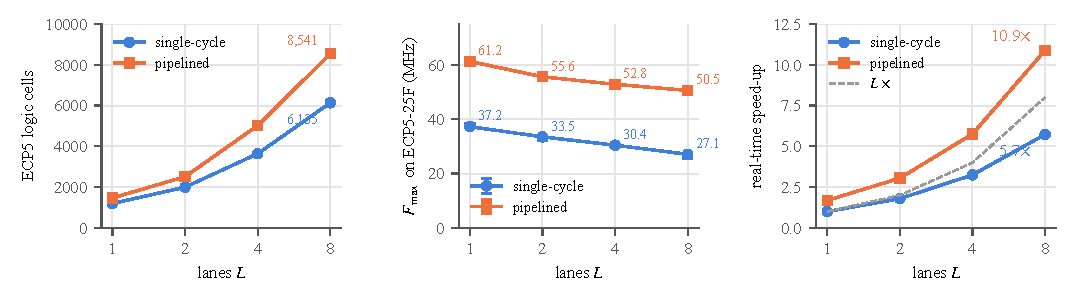
\includegraphics[width=\textwidth]{figures/p2_fpga.pdf}
\caption{Both cores on the ECP5-25F against lane count: logic cells after place and
route; $F_{\max}$, median of three placement seeds with the range; and real-time speed-up
over the single-cycle one-lane core, the mean over eight workloads of $N = 256$
elements (dashed: $L\times$).}
\label{fig:fpga2}
\end{figure*}

\subsection{FPGA Resources and Clock Frequency}
Table~\ref{tab:fpga2} and Fig.~\ref{fig:fpga2} give the results. Both cores were built
with the program that uses every instruction loaded, so no logic can be optimised away,
and each ECP5 build was placed three times. The pipeline raises $F_{\max}$ by $1.64\x$ at
one lane and $1.87\x$ at eight, and the clock falls more slowly with the lane count: by
17\% from one to eight lanes, against 27\% for the single-cycle core, because the adder
tree, which deepens with $L$, now has a stage of its own. The slowest path moves from a
whole instruction (instruction RAM to scalar register file) to a single stage: at one
lane the fetch loop, in which the decoded branch guess selects the next fetch address;
from two lanes on the execute stage, from a forwarded operand through the lane
multiplier into the X/W register, a path that widens with $L$ because the forwarding
multiplexers are $16L$ bits wide.

The price is logic: 39\% more ECP5 cells at eight lanes and about 300 flip-flops for the
pipeline registers. On Artix-7, whose six-input LUTs absorb the wide multiplexers better,
the increase is 7\% (3,600 against 3,372 LUTs). The Phase~II features also cost the
single-cycle core: with masks, \texttt{VMSK} and saturation it needs 6,135 cells and
reaches 27.1~MHz at eight lanes, against 5,396 cells and 29.1~MHz for the Phase~I build.
The comparison between the two cores is unaffected, since both implement the same
instruction set.

\begin{table}[t]
\centering
\caption{ECP5-25F after place and route (median $F_{\max}$ of 3 seeds)}
\label{tab:fpga2}
\footnotesize
\begin{tabular}{@{}llrrrl@{}}
\toprule
Core & $L$ & Cells & FFs & $F_{\max}$ & Slowest path \\
\midrule
single & 1 & 1,197 & 17  & 37.3 & I-RAM $\to$ vector regs \\
single & 8 & 6,135 & 24  & 27.1 & I-RAM $\to$ scalar regs \\
pipe   & 1 & 1,468 & 189 & 61.3 & I-RAM $\to$ I-RAM (fetch) \\
pipe   & 2 & 2,510 & 207 & 55.6 & X/W register (execute) \\
pipe   & 4 & 5,018 & 243 & 52.8 & X/W register (execute) \\
pipe   & 8 & 8,541 & 315 & 50.6 & W $\to$ X $\to$ W (execute) \\
\bottomrule
\end{tabular}
\end{table}

\subsection{Cycles and Where They Go}
Table~\ref{tab:cyc2} lists the cycle counts at eight lanes and Fig.~\ref{fig:cyc2}(a)
splits them into instructions and extra cycles. The two cores need almost the same
number of cycles, the pipelined core 0.4\% fewer on average, for different reasons. The
single-cycle core pays one extra cycle per load. The pipelined core pays nothing for
loads but one cycle whenever a loaded register, a reduction sum or a masked result is
used by the very next instruction, plus two fixed cycles (the pipeline fill and the
wrong guess at the loop exit). The balance per loop pass decides the difference: the
pipelined core needs 30 and 62 fewer cycles on \texttt{vadd} and \texttt{saxpy}, which
save more load cycles than they stall (\texttt{saxpy} never stalls); two more on
\texttt{relu}, \texttt{threshold}, \texttt{dot} and \texttt{brighten}, where every saved
load cycle becomes a stall; and 34 more on \texttt{abs} and \texttt{sumpos}, which stall
twice per pass but load only once. Counted in cycles, both cores still scale almost perfectly with the lanes:
the mean speed-up of eight lanes over one is $7.89\x$ for the single-cycle core and
$7.83\x$ for the pipelined one, whose fixed extra cycles do not shrink with $L$.

\begin{table}[t]
\centering
\caption{Cycles and time at 8 lanes, $N = 256$ (ECP5 $F_{\max}$)}
\label{tab:cyc2}
\footnotesize
\begin{tabular}{@{}lrrrrr@{}}
\toprule
 & \multicolumn{2}{c}{Cycles} & \multicolumn{2}{c}{Time ($\mu$s)} & Pipe \\
\cmidrule(lr){2-3}\cmidrule(lr){4-5}
Workload & single & pipe & single & pipe & speed-up \\
\midrule
\texttt{vadd}      & 259 & 229 & 9.57  & 4.53 & 2.11$\x$ \\
\texttt{saxpy}     & 292 & 230 & 10.79 & 4.55 & 2.37$\x$ \\
\texttt{relu}      & 195 & 197 & 7.21  & 3.90 & 1.85$\x$ \\
\texttt{threshold} & 261 & 263 & 9.65  & 5.20 & 1.85$\x$ \\
\texttt{dot}       & 260 & 262 & 9.61  & 5.18 & 1.85$\x$ \\
\texttt{brighten}  & 196 & 198 & 7.25  & 3.92 & 1.85$\x$ \\
\texttt{abs}       & 260 & 294 & 9.61  & 5.82 & 1.65$\x$ \\
\texttt{sumpos}    & 261 & 295 & 9.65  & 5.84 & 1.65$\x$ \\
\midrule
mean               &     &     &       &      & 1.90$\x$ \\
\bottomrule
\end{tabular}
\end{table}

\begin{figure*}[t]
\centering
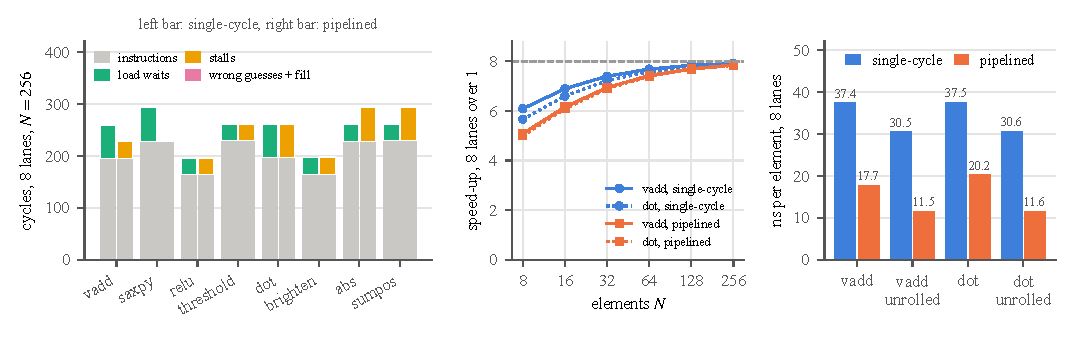
\includegraphics[width=\textwidth]{figures/p2_cycles.pdf}
\caption{(a) Cycles at eight lanes split into instructions and extra cycles (left bar of
each pair: single-cycle core; right: pipelined). (b) Cycle speed-up of eight lanes over
one against the problem size $N$, measured on the RTL. (c) Time per element at eight
lanes for the original loops and loops unrolled four times.}
\label{fig:cyc2}
\end{figure*}

\subsection{Real-Time Speed-Up}
Because the cycle counts are so close, the pipeline's advantage is its clock. In real
time it is $1.90\x$ faster than the single-cycle core at eight lanes
(Table~\ref{tab:cyc2}). Where stalls exactly replace saved load cycles the gain equals
the clock ratio, $1.85\x$ after the two fixed cycles; \texttt{vadd} and \texttt{saxpy}
gain more ($2.11\x$ and $2.37\x$), and \texttt{abs} and \texttt{sumpos}, with one
stall per pass more than they save, gain least ($1.65\x$). Against the scalar baseline, the single-cycle one-lane core, the
eight-lane single-cycle core is $5.73\x$ faster and the eight-lane pipelined core
$10.88\x$ (Fig.~\ref{fig:fpga2}, right). The pipelined core alone, at one lane, is
$1.68\x$ faster than the scalar baseline: pipelining and SIMD contribute separately, and
their product exceeds the lane count.

\subsection{Throughput and Area Efficiency}
Dividing the elements processed by the real time gives throughput, and dividing that by
the logic used gives area efficiency (Table~\ref{tab:eff}). At eight lanes the pipelined
core processes 53.8 million elements per second against 28.5 for the single-cycle core,
and 6.30 against 4.64 per thousand logic cells: the extra pipeline logic more than pays
for itself, so the pipelined core is the more efficient design at every lane count, not
only the faster one. For both cores efficiency is roughly flat with $L$, because the
lanes add logic and throughput almost in proportion while the shared control is a small
part of the total.

\begin{table}[t]
\centering
\caption{Throughput and area efficiency (mean of eight workloads)}
\label{tab:eff}
\footnotesize
\begin{tabular}{@{}rrrrr@{}}
\toprule
 & \multicolumn{2}{c}{M elements/s} & \multicolumn{2}{c}{per 1,000 cells} \\
\cmidrule(lr){2-3}\cmidrule(lr){4-5}
$L$ & single & pipe & single & pipe \\
\midrule
1 & 5.0  & 8.3  & 4.15 & 5.67 \\
2 & 8.9  & 15.1 & 4.47 & 6.00 \\
4 & 16.1 & 28.5 & 4.43 & 5.67 \\
8 & 28.5 & 53.8 & 4.64 & 6.30 \\
\bottomrule
\end{tabular}
\end{table}

\subsection{Problem Size}
Fig.~\ref{fig:cyc2}(b) shows the cycle speed-up of eight lanes over one for
$N = 8$ to $256$, measured on the RTL for \texttt{vadd} and \texttt{dot} on both cores
(Table~\ref{tab:size}). At $N = 8$ the eight-lane loop runs once, the setup code is a
large share of the work and the speed-up is $5.0$--$6.1\x$; by $N = 256$ it is within 2\%
of the ideal $8\x$. This is Amdahl's law with a serial fraction that shrinks as $N$
grows. The pipelined core falls slightly further at small $N$ because its fixed part,
which includes the pipeline fill and the final wrong guess, is larger.

\begin{table}[t]
\centering
\caption{Cycle speed-up of 8 lanes over 1 against problem size}
\label{tab:size}
\footnotesize
\begin{tabular}{@{}rrrrr@{}}
\toprule
 & \multicolumn{2}{c}{\texttt{vadd}} & \multicolumn{2}{c}{\texttt{dot}} \\
\cmidrule(lr){2-3}\cmidrule(lr){4-5}
$N$ & single & pipe & single & pipe \\
\midrule
8   & 6.09 & 5.08 & 5.67 & 5.00 \\
16  & 6.89 & 6.16 & 6.60 & 6.09 \\
32  & 7.40 & 6.94 & 7.22 & 6.89 \\
64  & 7.69 & 7.43 & 7.59 & 7.40 \\
128 & 7.84 & 7.70 & 7.79 & 7.69 \\
256 & 7.92 & 7.85 & 7.89 & 7.84 \\
\bottomrule
\end{tabular}
\end{table}

\subsection{Unrolling and Instruction Order}
Unrolling \texttt{vadd} and \texttt{dot} four times, with all eight loads placed first,
helps both cores but for different reasons. Both execute 25\% fewer instructions,
because the loop overhead is paid once per four vectors. Only the pipelined core also
loses its stalls: every register is loaded several instructions before it is used, and
in \texttt{dot\_unroll} each \texttt{VDOT} writes its own register, consumed four
instructions later. The pipelined core then completes one instruction per cycle
(147 instructions in 149 cycles for \texttt{vadd\_unroll}), and the time per element
falls from 17.7 to 11.5~ns for \texttt{vadd} and from 20.2 to 11.6~ns for \texttt{dot}
(Fig.~\ref{fig:cyc2}(c)). The unrolled programs on the eight-lane pipelined core are
$18.6\x$ faster than the original programs on the scalar single-cycle core, and
$15.1\x$ faster than the same unrolled programs there. The hardware
sets the clock; the order of the instructions decides how many clocks are wasted.

\subsection{Limitations}
$F_{\max}$ is nextpnr's static timing estimate without pin constraints; the design has
not run on a board, and the Vivado flow for the Basys-3, which would give exact Artix-7
timing, could not be run because Vivado does not support the development machine. Power
was not measured. Real time assumes a memory that delivers a 128-bit word per cycle, as
the on-chip block RAM does. The branch predictor is static, which suits these loops but
would mispredict data-dependent branches. One mask register and one element width keep
the encoding small; a wider multiply and \texttt{vsetvli}-style length control remain
open.

% =============================================================================
\section{Conclusion}\label{sec:conclusion}
Measuring the single-cycle core's critical path located its clock limit in three nearly
equal pieces, and a four-stage pipeline built around them raised the eight-lane clock
from 27.1 to 50.6~MHz. Forwarding, write-through register files, three one-cycle stall
rules and backward-taken branch prediction keep the cycle count within 0.4\% of the
single-cycle core, so the clock gain becomes a $1.90\x$ real-time gain, and the eight-lane
pipelined core is $10.9\x$ faster than the scalar single-cycle design ($18.6\x$ with
unrolled loops). Masked execution and saturating arithmetic bring the instruction set
closer to production SIMD extensions without a new register-file read port. A golden
model that predicts the cycle count of both cores made the pipeline verifiable to the
same standard as Phase~I: every workload, directed test, mid-run reset and random
program agrees with it, and every planted pipeline bug is caught. The remaining gains
lie in software (instruction scheduling) and in running the design on a board.

% =============================================================================
\section*{Code and Data Availability}
All RTL, testbenches, programs, scripts, results and figures are in the repository
named on the first page. \texttt{make test} runs the lint, unit testbenches, software
tests, both cores' system, directed, reset and random-program runs and the board checks;
\texttt{make fuzz} runs 8,000 random programs; \texttt{make perf}, \texttt{make sweep}
and \texttt{make syn} regenerate the cycle counts, the size sweep and the FPGA results;
and \texttt{make report} rebuilds the figures and this paper from them.

\section*{Individual Contributions}
\textbf{Mahir Abdullah} (lead): the critical-path analysis and the pipeline design; the
shared decoder, the pipelined core and the hazard unit; masked execution across both
cores; the golden model's cycle model for both cores; the hazard, mask, long-branch and
mid-run reset tests, the random-program fuzzer for both cores and the planted-bug
campaign; continuous integration, documentation and this report.

\textbf{Krishiv Gupta}: saturating \texttt{ADDS} and \texttt{SUBS} in the lane ALU, with
hand-checked saturation cases and clamp coverage in its testbench and the reference
model; the FPGA top that builds either core, the board checks of both cores, and the
ECP5 and Artix-7 sweep of both cores with the slowest-path report.

\textbf{Abhiman Singh}: per-lane write enables, the lane mask register and the
write-through option of the vector and scalar register files, with a testbench that
builds each file in both modes and checks them against a shadow model.

\textbf{Gogulamudi Jayadeep}: masked lane sums and lane flags in the result combiner,
verified at every lane count; and the speed-up analysis: real-time comparison of both
cores, cycle breakdown, problem-size sweep, unrolled programs and the figures.

\textbf{Ashish Kushwaha}: assembler support for the saturating, masked and
\texttt{VMSK} instructions with its tests, the \texttt{brighten}, \texttt{abs} and
\texttt{sumpos} programs, and full coverage of the new instructions in
\texttt{isa\_test}.
